\capitulo{5}{Aspectos relevantes del desarrollo del proyecto}
\label{cap:RelvAsp}
En este capítulo, se recogerán los aspectos que han determinado el desarrollo del proyecto. Tanto las ideas iniciales, como las finalmente implementadas, así como la motivación para tomar ciertas decisiones, y la manera en que se solucionaron los errores encontrados. 

\section{Inicio del proyecto}

La idea de este proyecto surgió al plantearme si quería pasar 12 créditos (300h) desarrollando algo que no me interesase ni motivase demasiado. Al fin y al cabo, 4 años de carrera deberían de acabar bien y, tal y como empezó, aprendiendo algo.

Así que se me ocurrió dar salida al \emph{drone} que construí hace casi 4 años, haciéndolo formar parte de mi proyecto de final de carrera. En principio mi idea era que el \emph{drone} recorriese un plano de un entorno abierto haciendo una ruta preestablecida. Grandes empresas del sector tecnológico (Amazon sobre todo) están jugueteando con la misma idea pero, generalmente por legislación, este proceso se está viendo muy lastrado. 

Me gustaba la idea. ¿Qué mejor forma de finalizar una carrera de ingeniería que hacer que un \emph{drone} se estrelle contra un obstáculo a alta velocidad, entre un amalgama de hélices y piezas hechas añicos? Al fin y al cabo, las pruebas son pruebas, y algo se iba  a romper sí o sí. Mejor si era de una forma espectacular.

El \cotutorOne{}, uno de mis tutores, no parecía tan seguro, ya habían jugueteado con algo parecido en el pasado (en un simulador), y no le apetecía pasar de nuevo por lo mismo. El mismo \cotutorOne{} sugirió la posibilidad de que el \emph{drone} actuase como un vigilante nocturno en la universidad, y el \cotutorTwo{} añadió que podría  hacer uso de un algoritmo de localización sin GPS. 

Además, nos harían falta conocimientos fuertes sobre hardware y mecanismos de control, y un tercer tutor siempre viene bien, entra el \tutor{}.

Y así comencé con el desarrollo de este proyecto que, en algún momento, tendrá el potencial suficiente como para convertirse en el \emph{sereno} de la Escuela Politécnica Superior de la Universidad de Burgos.

\begin{figure}
	\centering
	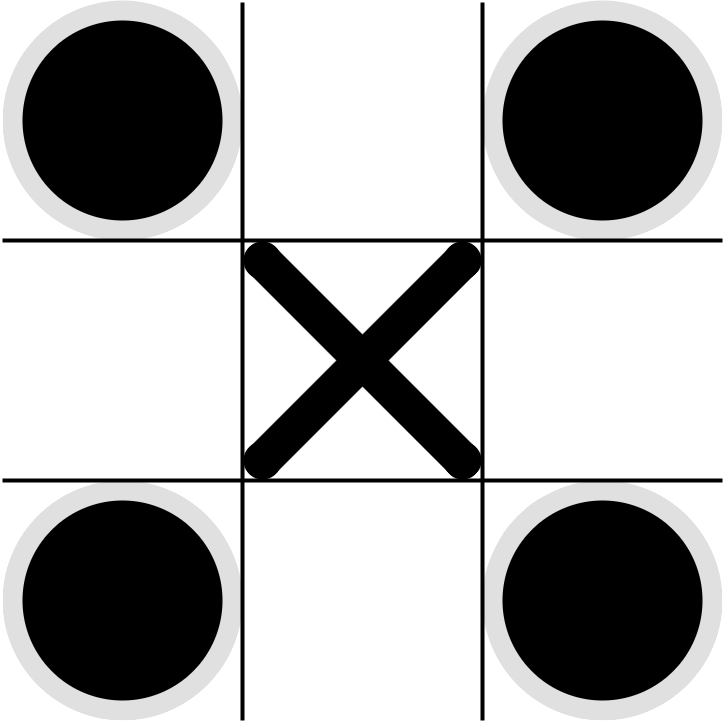
\includegraphics[width=0.5\textwidth]{Logo}
	\caption[Logo]{Logo de UBUDroneSereno.}\label{fig:Logo}
\end{figure}



\section{Metodología}

La gestión del proyecto se ha llevado a cabo a base de metodologías ágiles mediante \emph{Scrum}.
Sin embargo, cabe destacar que dado que el proyecto no se compone de varios integrantes, no es posible realizar en su totalidad el flujo de trabajo de Scrum, o este ha sido simplificado. 

\begin{itemize} 
\item Se han realizado iteraciones \emph{Sprint} bisemanales, en las que se han discutido las tareas a completar de cara a la siguiente reunión. 
\item Dichas tareas, denominadas \emph{Issues} han sido registradas haciendo uso de GitHub, que ha servido de plataforma de gestión de tareas y asignaciones. De nuevo, las asignaciones han sido realizadas por un único alumno. 
\item Se ha hecho uso de \emph{Kanban} mediante la implementación que ofrece ZenHub de un tablero para tarjetas, y de la herramienta Glo, disponible en GitKraken. 
\item El flujo de trabajo se ha distribuido mediante Kanban, en diferentes pilas (En progreso, Cerrada, Backlog, IceBox... etc).
\item Para comprobar el correcto ritmo de desarrollo del proyecto se ha hecho uso de los gráficos BurnDown que provee ZenHub, pero de nuevo, al no tratarse de un proyecto en el que intervienen múltiples desarrolladores, no es posible ajustarse al modelo presentado en los gráficos como ideal. 
\end{itemize}

Para el desarrollo de todas las partes del proyecto se ha seguido el mismo proceso: 
\begin{enumerate}
\item Se recaba toda la información necesaria para llevar a cabo la implementación.
\item Se estudia en profundidad la documentación.
\item Se comienza creando las clases de la implementación con una estrategia de diseño \emph{bottom-up}, aunque las clases de más alto nivel siguen una estrategia \emph{top-down} de forma que se requiere de una visión completa del proyecto para poder enlazarlas correctamente.
\end{enumerate}

No se ha seguido un diseño dirigido por pruebas, \emph{TDD}, ya que se ha considerado que genera una cantidad de código a refactorizar demasiado grande durante las etapas más tempranas, y dada la magnitud del proyecto solo conseguiría ralentizar el proceso de desarrollo. 
Se detallará más sobre las pruebas en la sección \ref{sec:testing}.


\section{Formación}

Para el desarrollo del proyecto se ha hecho uso de conocimientos adquiridos en la presente carrera, en muchos años de curiosidad y de búsqueda en internet. 

El desarrollo ha sido, en su mayor parte, escrito en Python, y se ha hecho uso de librerías como Numpy, Matplotlib y SciPy que se estudian durante la carrera, y otras que no, como PySerial (para establecer una comunicación serie), Bluetin-Echo (para hacer uso de los sensores de distancia HC-SR04), el framework Flask (para el desarrollo de la web-app) y la API WebRTC (para el vídeo en tiempo real) entre otras.

Sin embargo, cabe destacar la lectura de ciertos artículos, y el acceso a ciertos recursos:

\begin{itemize}
\item \textit{Artificial Intelligence for Robotics}. Un curso de Udacity impartido por Sebastian Thurn, disponible en \citep{wiki:UdCityPF}. En él se explican componentes habituales en múltiples proyectos, como el controlador PID, el filtro de Kalman, y otros no tan habituales, como el FIltro de Partículas utilizado en este proyecto para lograr un sistema de localización que no dependa de GPS, ver sección \ref{subsec:PF}.
\item MultiWiiSerialProtocol. Interfaz o definición del protocolo de comunicación MultiWii, utilizado en prácticamente todas las controladoras de vuelo actuales, como base de comunicación con ordenadores. Este protocolo es el utilizado para comunicar la RaspberryPi con la controladora de vuelo, y enviar/recibir comandos. Disponible en \citep{wiki:MSPDefinition}.
\item \emph{Getting Started with WebRTC}, un compendio de las funcionalidades que ofrece WebRTC para lograr comunicación en tiempo real. Utilizado para lograr vídeo sin apenas latencia entre un navegador y la RaspberryPi a bordo del \emph{drone}. Disponible en \citep{wiki:WebRTCFullDesc}.
\item \emph{The Vector Field Histogram - Fast Obstacle Avoidance for Mobile Robots}. Se trata del artículo original de Borenstein y Koren, en el que detallan el funcionamiento del sistema de evasión de obstáculos implementado. Disponible en \citep{art:BorensteinKorenVFH}.
\item \emph{The Flask Megatutorial}. Miguel Grinberg da una clase magistral sobre como empezar, continuar y finalizar con Flask. Este mega-tutorial contiene todo lo necesario para preparar una web-app con Flask. Disponible en \citep{wiki:Flask}.
\end{itemize}

Por supuesto cabe destacar la ingente documentación disponible de Python, y todas las librerías que lo componen.
Sin duda hay muchas otras fuentes de formación relacionada con este proyecto, y pueden ser consultadas en la bibliografía. 



\section{Desarrollo de algoritmos}

En el desarrollo de este proyecto, se ha llevado a cabo el desarrollo de tres algoritmos fundamentales: 

\begin{itemize}

\item Un sistema de evasión de obstáculos. Llevado a cabo mediante la implementación de dos algoritmos: el algoritmo de Campos Potenciales, y el algoritmo VFH en sustitución del primero.
\item Un sistema de localización sin depender de la red de satélites GPS/Glonass. Llevado a cabo mediante la implementación de un Filtro de Partículas basado en simulación de Montecarlo, para estimar la variable \emph{posición}, en base a las variables \emph{distancias a obstáculos}.
\item Varios controladores automatizados para complementar la evasión de obstáculos, y lograr la autonomía del sistema. Llevados a cabo mediante implementaciones de controladores PID, alimentados por la salida del algoritmo VFH, y por las lecturas de los sensores de la controladora de vuelo (para la inclinación) y un sensor de ultrasonidos colocado para medir la altura del \emph{drone}.
\end{itemize}

\subsection{Potential Fields}

Durante el primer Sprint, y mientras decidíamos que algoritmos deberíamos usar para lograr el propósito del proyecto, el \tutor{} sugirió la utilización del algoritmo de Campos Potenciales para llevar a cabo la evasión de obstáculos.

El algoritmo de campos potenciales se basa en la idea de que existe una meta a la que se quiere llegar, y una serie de obstáculos. 

La meta genera una fuerza de atracción sobre el \emph{drone}, y los obstáculos fuerzas repulsoras. 
En primera instancia este algoritmo es relativamente sencillo de implementar, y no tiene un coste computacional muy alto. Toda la dimensionalidad del problema se acaba reduciendo a una suma de fuerzas, que determinan el vector resultante, con una dirección y un sentido que el \emph{drone} deberá seguir. 

Sin embargo, este método presenta ciertos inconvenientes:
\begin{itemize}
\item Si el \emph{drone} entra en una zona con forma de `U', podría atascarse en un mínimo local, entrando y saliendo de ella indefinidamente. 
\item Una zona estrecha es todo un desafío. Las paredes de un pasillo, por ejemplo, presentan fuerzas repulsoras sobre el \emph{drone}, y la fuerza atrayente de la meta no es suficiente como para mantener la dirección del \emph{drone} a través del pasillo, con lo que este empezará a oscilar (si es que ha conseguido entrar en él) o ni siquiera será capaz de pasar de la entrada del pasillo.
\end{itemize}

Por ello se ha hecho uso del Vector Field Histogram.

\subsection{Vector Field Histogram}
\label{subsec:VFHcomments}
El Vector Field Histogram se basa en el uso de una malla de certidumbre. Dicha malla es una representación del plano, el cual se divide en celdas (muy apropiado para usarlo con Numpy, y aprovechar la potencia del cálculo vectorizado de que provee). 

Cada celda contiene un valor, dicho valor es la certeza de que en ella exista un obstáculo. Por tanto se define un tamaño para las celdas ($5 \times 5$ cm es una buena medida teniendo en cuenta el rango de detección de nuestros sensores de ultrasonidos), y se realizan medidas mediante los sensores de ultrasonidos. 

Encontrar un obstáculo en cierta posición supone incrementar en 1 la cuenta que existe en la celda que representa esa distancia del agente. 
Computacionalmente, este método supera al algoritmo de Campos Potenciales, ya que no es necesario tener en cuenta en que posición del rayo que dispara el sensor (recordemos de la documentación teórica que el HC-SR04 tiene una amplitud de unos 30º), creando una distribución Gaussiana alrededor de la bisectriz del rayo, sino que únicamente se incrementa la posición central. 

Puede parecer una sobresimplificación del problema, pero lo cierto es que tras múltiples medidas de los sensores disponibles, las malla de certidumbre representa con bastante fidelidad el estado del entorno cercano al \emph{drone}. 

Una vez obtenida la malla, esta se convierte en un histograma polar. Para ello se divide esta en sectores de una amplitud determinada (5º se ha mostrado como una cantidad aceptable, generando así 72 sectores que cubrirán los 360º). De esta forma, ya se dispone de una representación aproximada de la ubicación de los obstáculos. 

Aún así se somete el histograma a una función de suavizado. En el artículo presentado por Borenstein y Koren en \citep{art:BorensteinKorenVFH}, la función utilizada contiene una errata. Tras discutirlo con mis tutores, decidimos utilizar cualquiera de las funciones de suavizado o filtrado disponibles en SciPy, tal y como sugirió el \cotutorTwo{}, y me decanté por la señal de Hann. 
De esta forma, los obstáculos parecen \textit{estirarse}, ya que la señal de Hann permite establecer la simetría de los valores a suavizar. Así que la certidumbre sobre la existencia de obstáculos en un punto contiguo a los obtenidos en la malla de certidumbre se verá incrementada, creando un histograma todavía más conservador sobre la posición de los obstáculos. 

Por si esto pudiera parecer poco, se define un umbral. El umbral establece cual es el nivel máximo de certidumbre de obstáculos en una zona, como para considerarla segura para navegar. 
El histograma presenta una serie de subidas y bajadas, como valles y colinas. Los valles, son precisamente las zonas que, umbral mediante, serán seguras para navegar.

Una vez obtenidos los valles (compuestos de varios sectores seguros), el algoritmo establecerá cual es el sector elegido para dirigirse a él, en base a la ubicación de la meta a la que se quiere llegar. 
Precisamente en este paso se determina la fortaleza de este método frente a los Campos Potenciales. El VFH va a elegir siempre el centro del valle para navegar, de forma que puede navegar en zonas estrechas, siempre que el umbral lo permita. 

Y precisamente en este paso es donde se encuentra otro problema en el artículo de Borenstein y Koren en \citep{art:BorensteinKorenVFH}, si siempre se elige el sector central para navegar, en el momento en el que se sale de una región estrecha (un pasillo por ejemplo) y la meta no está en el centro, el \emph{drone} empezará a ejecutar un movimiento circular aproximándose a la meta en un movimiento cada vez más cerrado pero, matemáticamente, puede que infinito. Por ello, se incluyó una modificación en el algoritmo original, que permite aproximarse al destino de forma directa, si este se encuentra a la vista del \emph{drone}, esto es, en un sector seguro para su navegación.

La salida del algoritmo se ha codificado como la orientación que el \emph{drone} debería seguir, es decir, presenta un valor en el intervalo $[-179, 180]$, el cual expresa cuantos grados debería rotar el \emph{drone}, y dado el signo la dirección de rotación, para dirigirse a la meta a través de un sector seguro. 
Además, el VFH, proporciona una medida de la velocidad que debería alcanzar el \emph{drone}, en base a como de ocupado está el sector en el que el \emph{drone} navega. La velocidad será proporcionada en base a la certidumbre de obstáculos, de manera que se irá reduciendo para poder realizar un cambio de sentido.

Este valor, por si solo, no es de mucha utilidad ya que no es interpretable por la controladora de vuelo, sino que tiene que ser \textit{convertido} a un valor entre $[1000, 2000]\mu s$. Para ello, se ha hecho uso de controladores PID, ver \ref{subsec:PIDcomments}.

\subsection{Particle Filter}
\label{subsec:PFcomments}
El Filtro de Partículas es una pieza clave en el funcionamiento del proyecto. Provee de información sobre la posición del agente de forma muy robusta, ya que está basado en un modelo probabilístico que obtiene sus valores mediante un método de Montecarlo. 

Básicamente, el algoritmo crea \emph{drones virtuales} (partículas) que obtienen medidas hasta los obstáculos. Conociendo esas medidas, y comparándolas con las del \emph{drone} real, parece inmediato poder decir cuanto se parece un \emph{drone virtual} al \emph{drone} real, y establecer esa posición como la posición del \emph{drone}. 

Y por supuesto, en teoría casi todo es sencillo: los diferentes cursos, artículos, páginas web y tutoriales basados en teoría, siempre hablan de \emph{landmarks}. Estos \emph{landmarks}, son zonas reconocibles por el agente (una diana en una pared, una marca... etc), predispuestas sobre el entorno, de manera que tanto las partículas como el agente pueden medir sus distancias a ellos, y de esta forma calcular como de parecidas son las partículas al agente. 

Sin embargo, a la hora de la práctica, no hay tales \emph{landmarks}. Por el sencillo hecho de que si tu agente no tiene al alcance alguno de esos \emph{landmarks}, no es nada probable que pueda medir su distancia a este. Pero sí tenemos paredes. 

Así que lo que se hace es calcular las distancias teóricas de cada una de las partículas a los obstáculos dentro de su área de acción (basada en la distancia máxima alcanzable por los sensores HC-SR04), con la esperanza de que no haya zonas simétricas ya que adquirirían la misma probabilidad de ser la zona en la que se encuentra el \emph{drone}.

El \emph{drone} por su parte toma medidas de las distancias, y se comparan las medidas reales con las de todas las partículas. 

El \emph{drone} se desplaza, y las partículas con él. Cada vez que el \emph{drone} hace un movimiento las partículas deben ejecutar ese mismo movimiento. Sencillo. Sí, en teoría. El \emph{drone} no gira o se desplaza la cantidad de grados o centímetros que se le ordena en cuanto se le ordena, el giro o el desplazamiento lleva tiempo. ¿Cuánto tiempo? No es nada sencillo de aproximar, depende del estado de la batería, de la temperatura (los ESC del \emph{drone} pueden llegar a reducir la velocidad de giro del motor si notan demasiado calor, aunque no es habitual), del cálculo de los controladores PID... etc. 
Es decir, existe una incertidumbre MUY grande, sobre todo en el desplazamiento. El movimiento de rotación es más sencillo de aproximar dado que se dispone de un magnetómetro, aunque tampoco es fiable al 100\% ya que puede estar alterado por la desviación magnética, diferente en cada punto del planeta, por la presencia de fuentes de magnetismo (motores, 4 en este caso), o fuentes de corriente elevadas (una batería alimentando 4 motores, por ejemplo).

De manera que se incluye cierta incertidumbre en cualquier movimiento realizado por las partículas, de esta forma la población de partículas va divergiendo, y alejándose poco a poco de la posición exacta del \emph{drone}, en su mayoría. 

Debido a ello, la población cada vez es menos útil al propósito de localización, así que se seleccionan individuos en base a la probabilidad de ser la posición real del agente. 
La selección se realiza con remplazo, es decir, una misma partícula puede aparecer varias veces. De esta forma la población vuelve a converger. 

Y con esto ya se dispondría de una ubicación aproximada para el \emph{drone}. Conocer la posición es fundamental para el funcionamiento del sistema de evasión de obstáculos, ver subsección \ref{subsec:VFHcomments}, dado que el VFH trata de guiar el \emph{drone} hacia la meta en una ruta segura, ¿cómo sabe hacia donde debe dirigir el \emph{drone}, si no sabe dónde se encuentra?

De esto se puede extraer una lección de lo más filosófica: primero descubre donde estas, para luego poder dirigirte hacia tu meta.


\subsection{PID}
\label{subsec:PIDcomments}
Para llevar a cabo el control automatizado del \emph{drone}, no es suficiente con proporcionar la salida de los diferentes algoritmos a la controladora de vuelo. 

La controladora de vuelo entiende entradas en sus canales (Acelerador, Inclinación, Balanceo, Rotación, Armar/Desarmar) en el intervalo $[1000, 2000]\mu s$, de manera que recibiendo la información proveniente de algunos sensores, se han creado los siguientes controladores PID: 

\begin{itemize}
\item Control de Altitud: Es fundamental disponer de un mecanismo de control constante de la altitud. Se alimenta de la información proveniente de un sensor de ultrasonidos que mira hacia el suelo, de forma que se puede establecer la altitud que debe alcanzar el \emph{drone}, relativa al suelo sobre el que se encuentra. Se encarga del canal 1, o Acelerador.
\item Control de Orientación: Este controlador se encarga de dirigir al \emph{drone} por el entorno, mediante cambios en su orientación. Se alimenta de la salida del VFH, ver subsección \ref{subsec:VFHcomments}, para establecer su objetivo, y del magnetómetro para establecer la medida real, y así crear una salida entre $[1400, 1600]\mu s$.
Esta salida es debida a la posición central del canal, $1500\mu s$, estableciendo la \emph{no} rotación del \emph{drone} en ningún sentido. Se encarga del canal 4, o Rotación.
\item Control de Velocidad: Este controlador se encarga de controlar la inclinación del \emph{drone}. No es posible determinar una velocidad concreta para el desplazamiento, dado que es muy variable, pero sí se puede establecer la inclinación que debe alcanzar el \emph{drone}. Esta inclinación es generada en base a los obstáculos en el sector en que se navega, y provista por el VFH, ver subsección \ref{subsec:VFHcomments}. De forma que tanto el objetivo, como el ajuste a realizar están automatizados. Genera una salida entre $[1400, 1600]\mu s$. La medida actual de la inclinación puede obtenerse de la controladora de vuelo. Se encarga del canal 2, o Elevación.
\end{itemize}


\section{Comunicaciones}

En el desarrollo de este proyecto, se ha llevado a cabo el desarrollo de tres sistemas de comunicación: 

\begin{itemize}
\item Un sistema de comunicación entre un ordenador y un \emph{drone}. Llevado a cabo mediante la librería de implementación propia \emph{MSPio}.
\item Un sistema de control remoto de un \emph{drone} a través de un navegador web. Llevado a cabo mediante Flask, Python y la librería MSPio.
\item Un sistema de vídeo en tiempo real. Llevado a cabo mediante la API de WebRTC, HTML, JavaScript, y en la parte del servidor (la RaspberryPi) se ha hecho uso de UV4L, un driver que accede a la cámara de la Raspberry, y provee de un servidor WebRTC al que conectarse, puede consultarse la web del proyecto en \citep{wiki:uv4l}.
\end{itemize}

\subsubsection{MSPio}

En este proyecto, la RaspberryPi no consta de un sistema de tiempo real y, por lo tanto, no es lo ideal para llevar a cabo el control de un sistema de tiempo real como lo es un \emph{drone}. De esta manera, se ha relegado esta tarea en una controladora de vuelo. 

Las controladoras de vuelo actuales, en su mayoría, implementan un mecanismo de comunicación con un ordenador para su configuración. 
Dicha configuración se realiza a través de una aplicación que muestra toda la parametrización que puede ser llevada a cabo (parámetros de PID, canales de radio, protocolos de radio, telemetría, alarmas, calibración, etc).

El protocolo que utilizan dichas controladoras de vuelo es generalmente el mismo: MultiWii Serial Protocol. 
Este protocolo se hereda de las primeras versiones de controladoras de vuelo, basadas en los mandos de la consola Wii de Nintendo\footnote{Wii y Nintendo son marcas registradas de Nintendo Co. LTD}, y de ahí su nombre.
La definición del protocolo es pública, así que cualquiera puede crear una implementación. 

Para este proyecto, se ha creado una implementación para Python 3.x, a la que se ha llamado MSPio.
Esta implementación es totalmente genérica, y permite el envío de órdenes a la controladora de vuelo, entre ellas la entrada de los canales que permiten mover el \emph{drone}, así como la solicitud de información, como inclinación, estado de la batería, temperatura, etc.

Para mayor comodidad, se han creado varios métodos que permiten la obtención de información, o el envío de los canales de radio como una lista de valores, con tan solo llamarlos. Aún así, se ha determinado como \emph{genérico}, ya que se ha definido el \emph{parseo} de los valores de respuesta de la controladora de vuelo, como una cadena de texto.
De forma que implementar la adquisición de nuevos datos es tan sencillo como pasar como parámetro una cadena de texto que representa la estructura de retorno. Ver tabla \ref{tb:MSP_MESSAGES}.

\subsubsection{Control Remoto}

El mecanismo de control remoto se ha llevado a cabo mediante un navegador web, dado que proporciona un acceso sencillo y sin barreras a cualquier usuario. 

Tan sencillo como iniciar sesión, el sistema establece qué \emph{drone} tiene asignado el usuario, y le conecta con él. La interfaz web permite la visualización en tiempo real de la emisión de vídeo disponible en el \emph{drone}, a traves de WebRTC, y su control con tan solo conectar una emisora al puerto USB del ordenador. 

Una vez conectada la emisora, la web reconoce la misma como un joystick, y es capaz de leer los canales, y enviarlos al servidor remoto, el cual los convierte en valores aceptables para el \emph{drone}, y se los envía a este a través de una comunicación socket.
Para activar el control remoto basta con activarlo y el \emph{drone} ya estará listo para ser controlado.

De esta manera, el usuario final no tiene una comunicación directa con el \emph{drone}, sino que el servidor intermedio es quien se encarga de esta tarea. 

Esto libera a la RaspberryPi de hospedar un servidor web y recibir clientes, así como del uso de un canal de comunicación potencialmente no seguro entre el cliente y el \emph{drone}. 


\begin{figure}
	\centering
	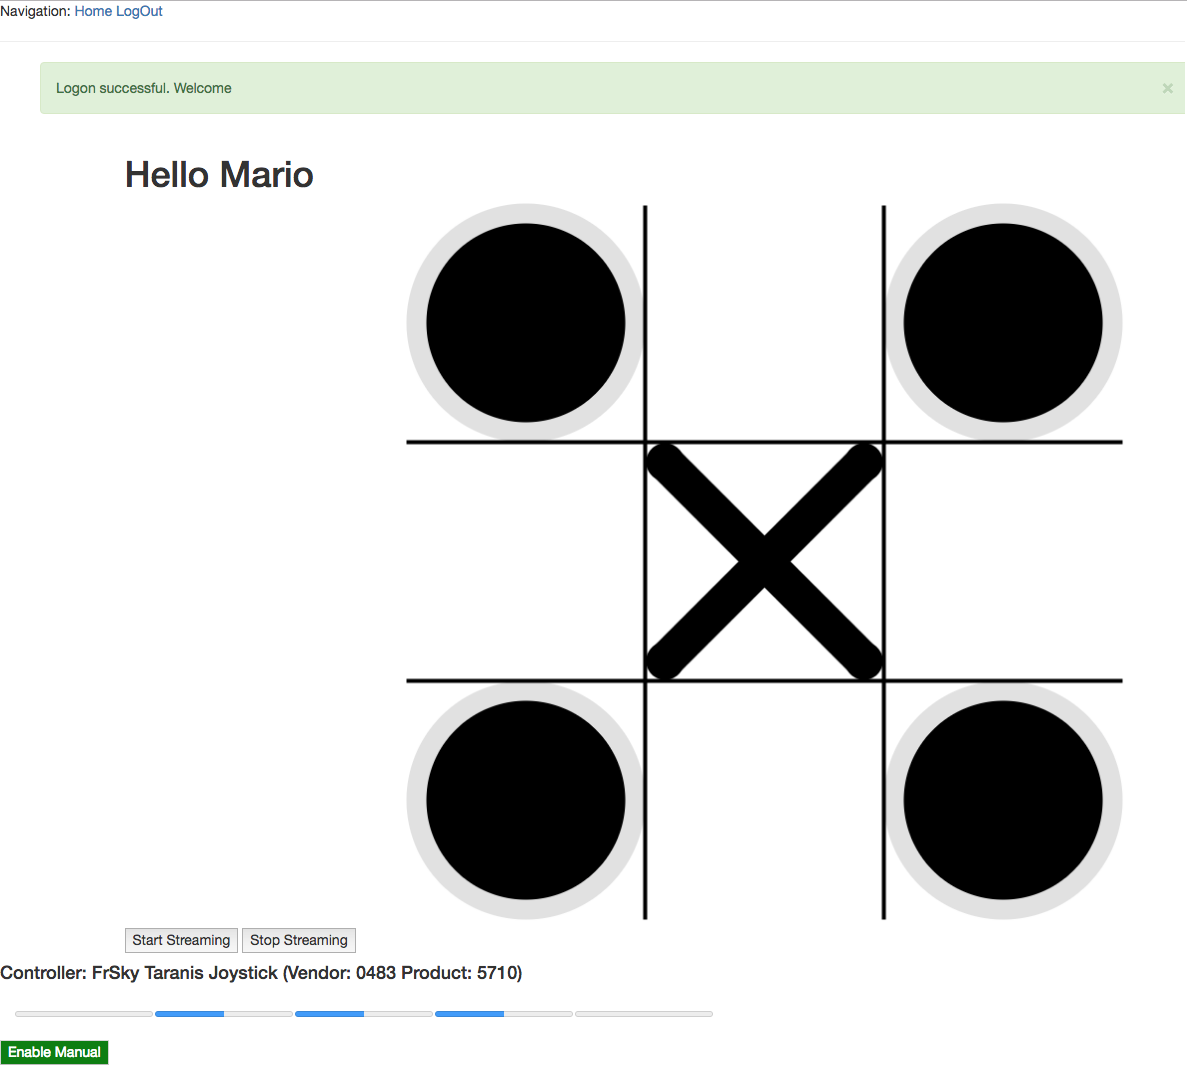
\includegraphics[width=0.9\textwidth]{webMain}
	\caption[Web index]{Página principal de la aplicación.}\label{fig:webmain}
\end{figure}

\subsubsection{Vídeo en Tiempo Real}

Integrar vídeo en una página web puede parecer trivial, pero no lo es en absoluto. Los contenedores existentes en HTML requieren que el vídeo esté finalizado para poder reproducirlo (MP4/WebM deben definir la duración del vídeo), lo cual ha dado varios quebraderos de cabeza. 

Se barajaron múltiples posibilidades, entre ellas:
\begin{itemize}
\item Hacer uso de MJPEG (Motion JPEG) consistente en tomar gran cantidad de fotografías e ir actualizando un canvas con cada nuevo fotograma. Sencillo, y simple de implementar, pero de un coste computacional inasumible dada la cantidad de trabajo que debe desempeñar la RaspberryPi.
\item Hacer uso de MPEG-DASH (Dynamic Adaptive Streaming over HTTP), pero se mostró como una solución con un coste computacional elevado, dado que suponía instalar el servidor en la RaspberryPi, hacer que este realizase streaming y que el servidor principal actuase como un repetidor para los usuarios.  
\end{itemize} 

Finalmente nos decantamos por WebRTC, dado que permite establecer una comunicación directa entre dos navegadores, sin necesidad de hacer uso de HTTP. El problema que plantea es que se trata de una API para trabajar entre navegadores, y no es elegante ni fiable mantener una navegador constantemente abierto en la RaspberryPi, dado que requiere de intervención del usuario para permitir acceso a la cámara. 
La solución pasaba por utilizar, o implementar, un servidor WebRTC, que implementase el protocolo \emph{Session Description Protocol} para comunicar un navegador cliente con la RaspberryPi. Por no añadir más carga de trabajo se ha hecho uso de UV4L, el cual es precisamente eso, un servidor que implementa las funcionalidades necesarias para hacer uso de WebRTC.

\section{Plataforma de usuario}

El manejo del \emph{drone} por parte del usuario se ha diseñado para ser de tremenda simplicidad. 
Tan solo se muestra una página de login, tal y como se muestra en la Figura \ref{fig:login}, que permite al usuario iniciar sesión. 

\begin{figure}
	\centering
	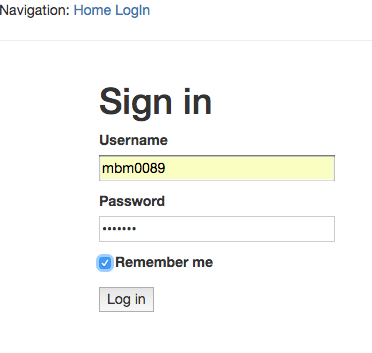
\includegraphics[width=0.7\textwidth]{loginWeb}
	\caption[Página de Login]{Página de inicio de sesión para los usuarios.}\label{fig:login}
\end{figure}

Una vez registrado en el sistema, se le muestra una interfaz que permite iniciar o detener el streaming de vídeo por parte del \emph{drone}. De esta forma, la RaspberryPi solo activa el servidor de vídeo cuando este se está visualizando, tal y como puede verse en la Figura \ref{fig:vidStream}. 
\begin{figure}
	\centering
	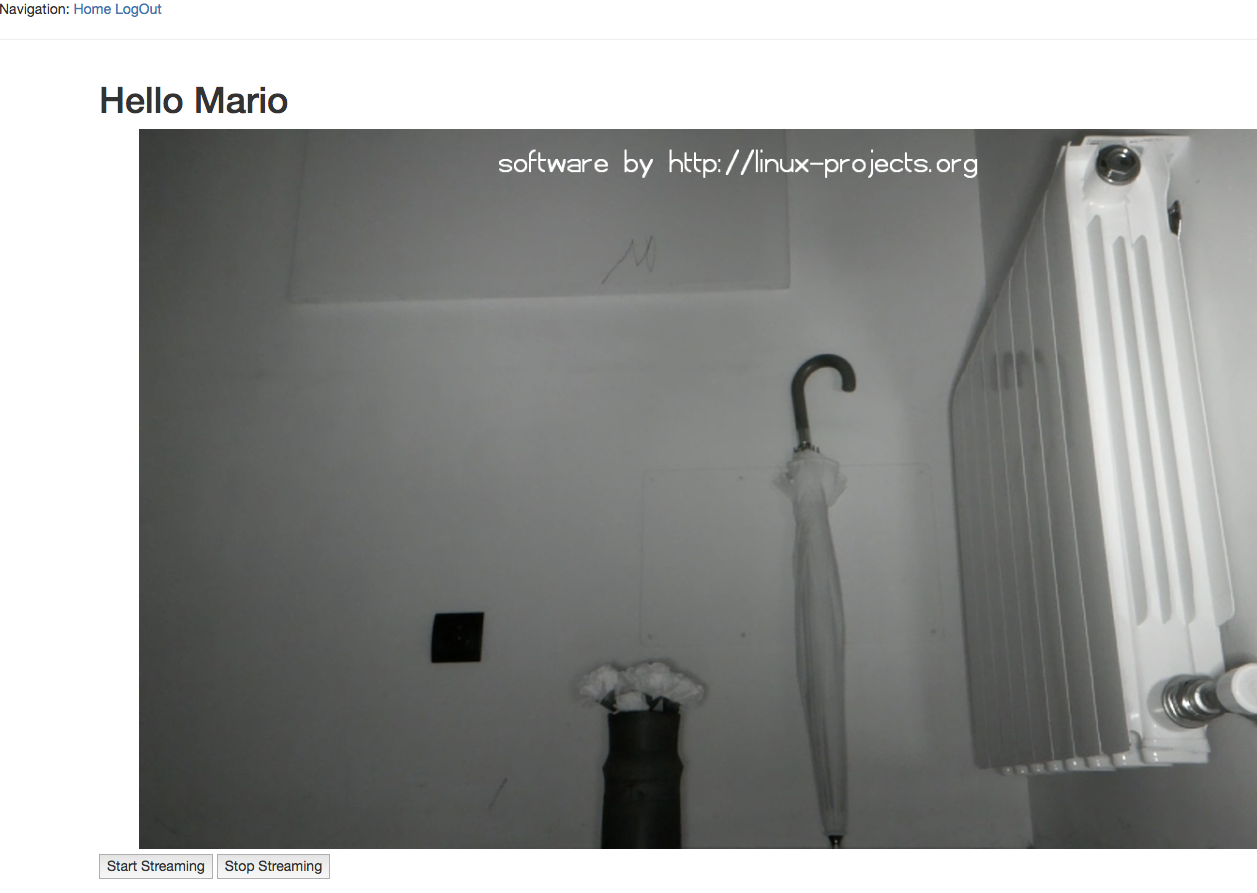
\includegraphics[width=0.7\textwidth]{vidStream}
	\caption[Página de control]{Página de del \emph{drone} asignado para los usuarios.Los LED IR están activos dada la condición de baja luminosidad.}\label{fig:vidStream}
\end{figure}

De conectar una emisora al equipo mientras el navegador está seleccionado, se reconoce ésta y permite controlar el \emph{drone} con tan solo pulsar un botón, tal y como puede verse en la Figura \ref{fig:fullConn}.

\begin{figure}
	\centering
	\includegraphics[width=0.7\textwidth]{fullConn}
	\caption[Página de control y emisora]{Página del \emph{drone} asignado para los usuarios lista para activar el control.}\label{fig:fullConn}
\end{figure}

La interfaz ha sido desarrollada en HTML5 y JavaScript, y la aplicación web se basa en el framework Flask, con la intención de aprender un nuevo medio de desarrollo de aplicaciones, y continuar trabajando con Python. 



\section{Hardware empleado}

El equipamiento empleado en el \emph{drone} es el siguiente: 

\begin{itemize}
\item Un \emph{drone} de 450mm de diagonal, distancia medida de motor a motor. Equipado con motores de 810KV (810rpm/V), controladores de velocidad (ESC) de 20A, una controladora de vuelo Flip32 con acelerómetro, giróscopo, magnetómetro y barómetro. Las hélices empleadas son de 9$"$ de longitud y 4.5$"$ de paso, generando un empuje máximo de 3.8Kg.
\item Una batería LiPo de 3700mAh y 35C (\emph{C} es la capacidad de descarga de la batería, en este caso sería $35 \times 3700mAh = 129500mAh = 129.5A$ máximo).
\item Seis sensores de ultrasonido HC-SR04. Cinco para las distancias a obstáculos y uno para controlar la altitud.
\item Una RaspberryPi 3B.
\item Una cámara PiNoIR. Sin filtro de infrarrojos, lo que permite el uso de LEDs infrarrojos para visión nocturna.
\item Dos anillos de LED infrarrojos para visión nocturna.
\item Seis divisores de voltaje para reducir el voltaje de salida de los sensores, ya que la RaspberryPi funciona a 3.3V y los sensores a 5V.
\item Cables para conectar todo.
\end{itemize}

\begin{figure}
	\centering
	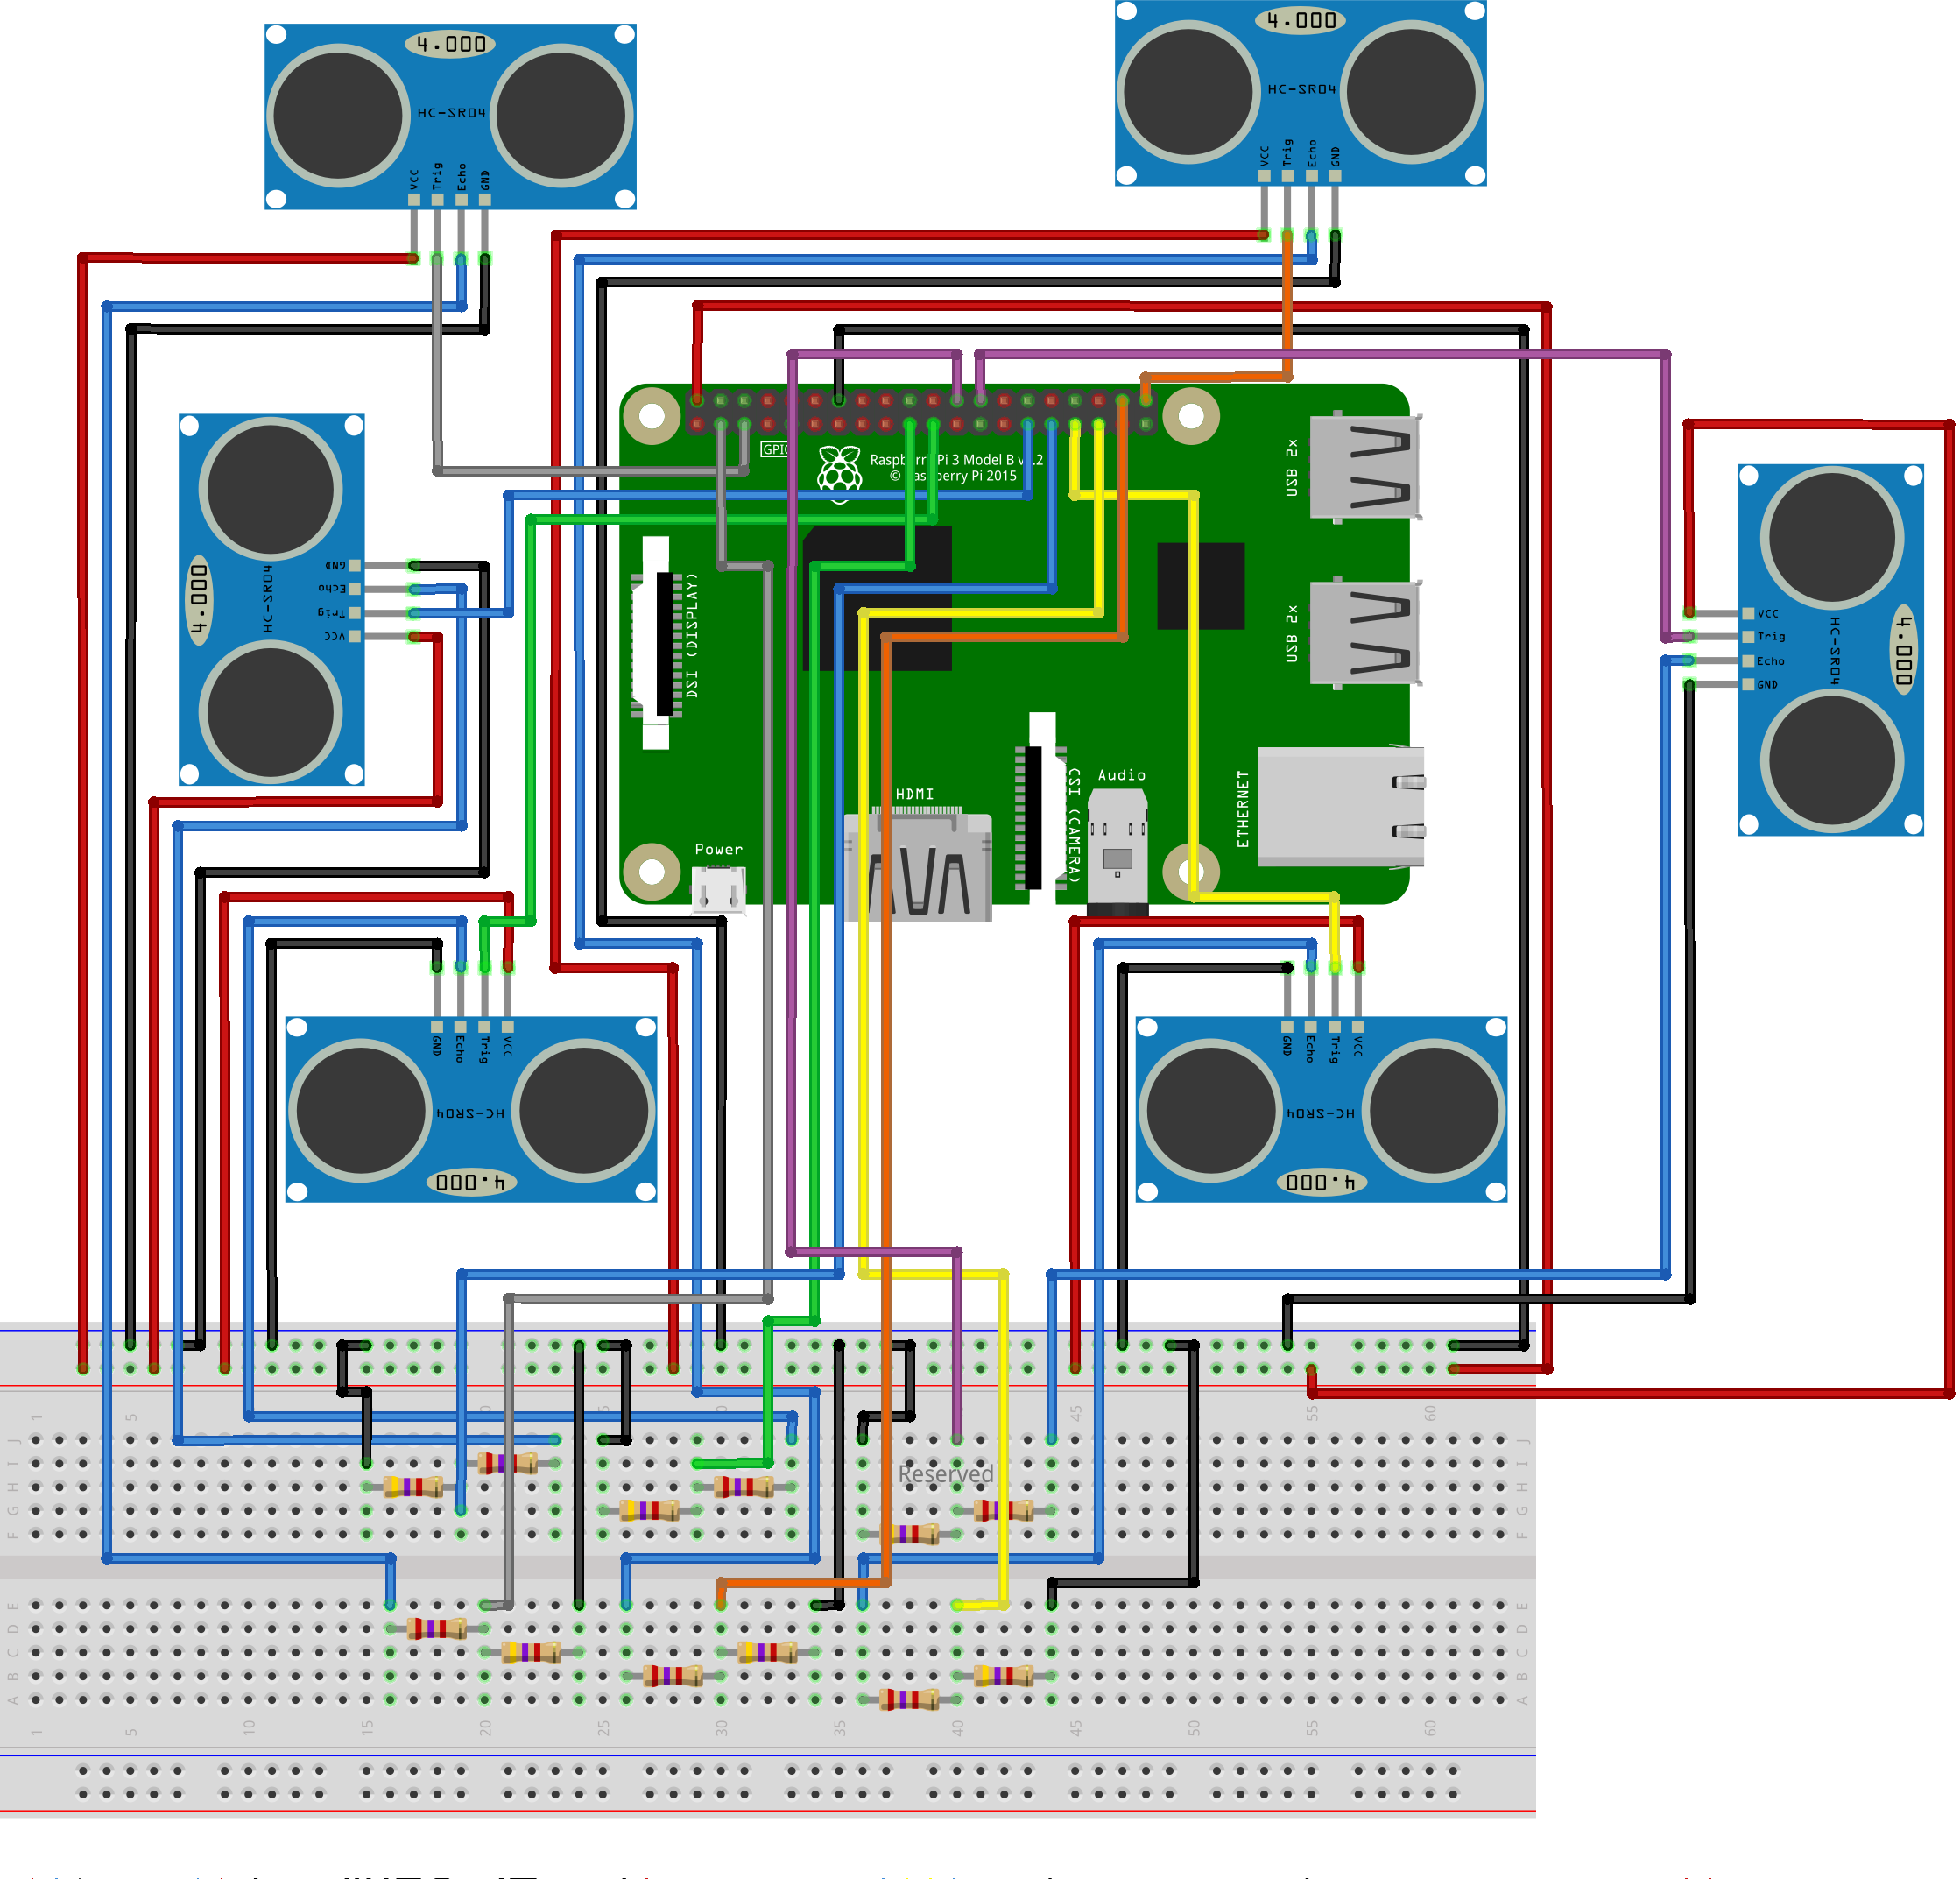
\includegraphics[width=0.9\textwidth]{SR04layout_bb}
	\caption[Conceptual de conexión de sensores a RaspberryPi]{Vista conceptual del conexionado de los sensores a la RaspberryPi.}\label{fig:schHCPi}
\end{figure}

\begin{figure}
	\centering
	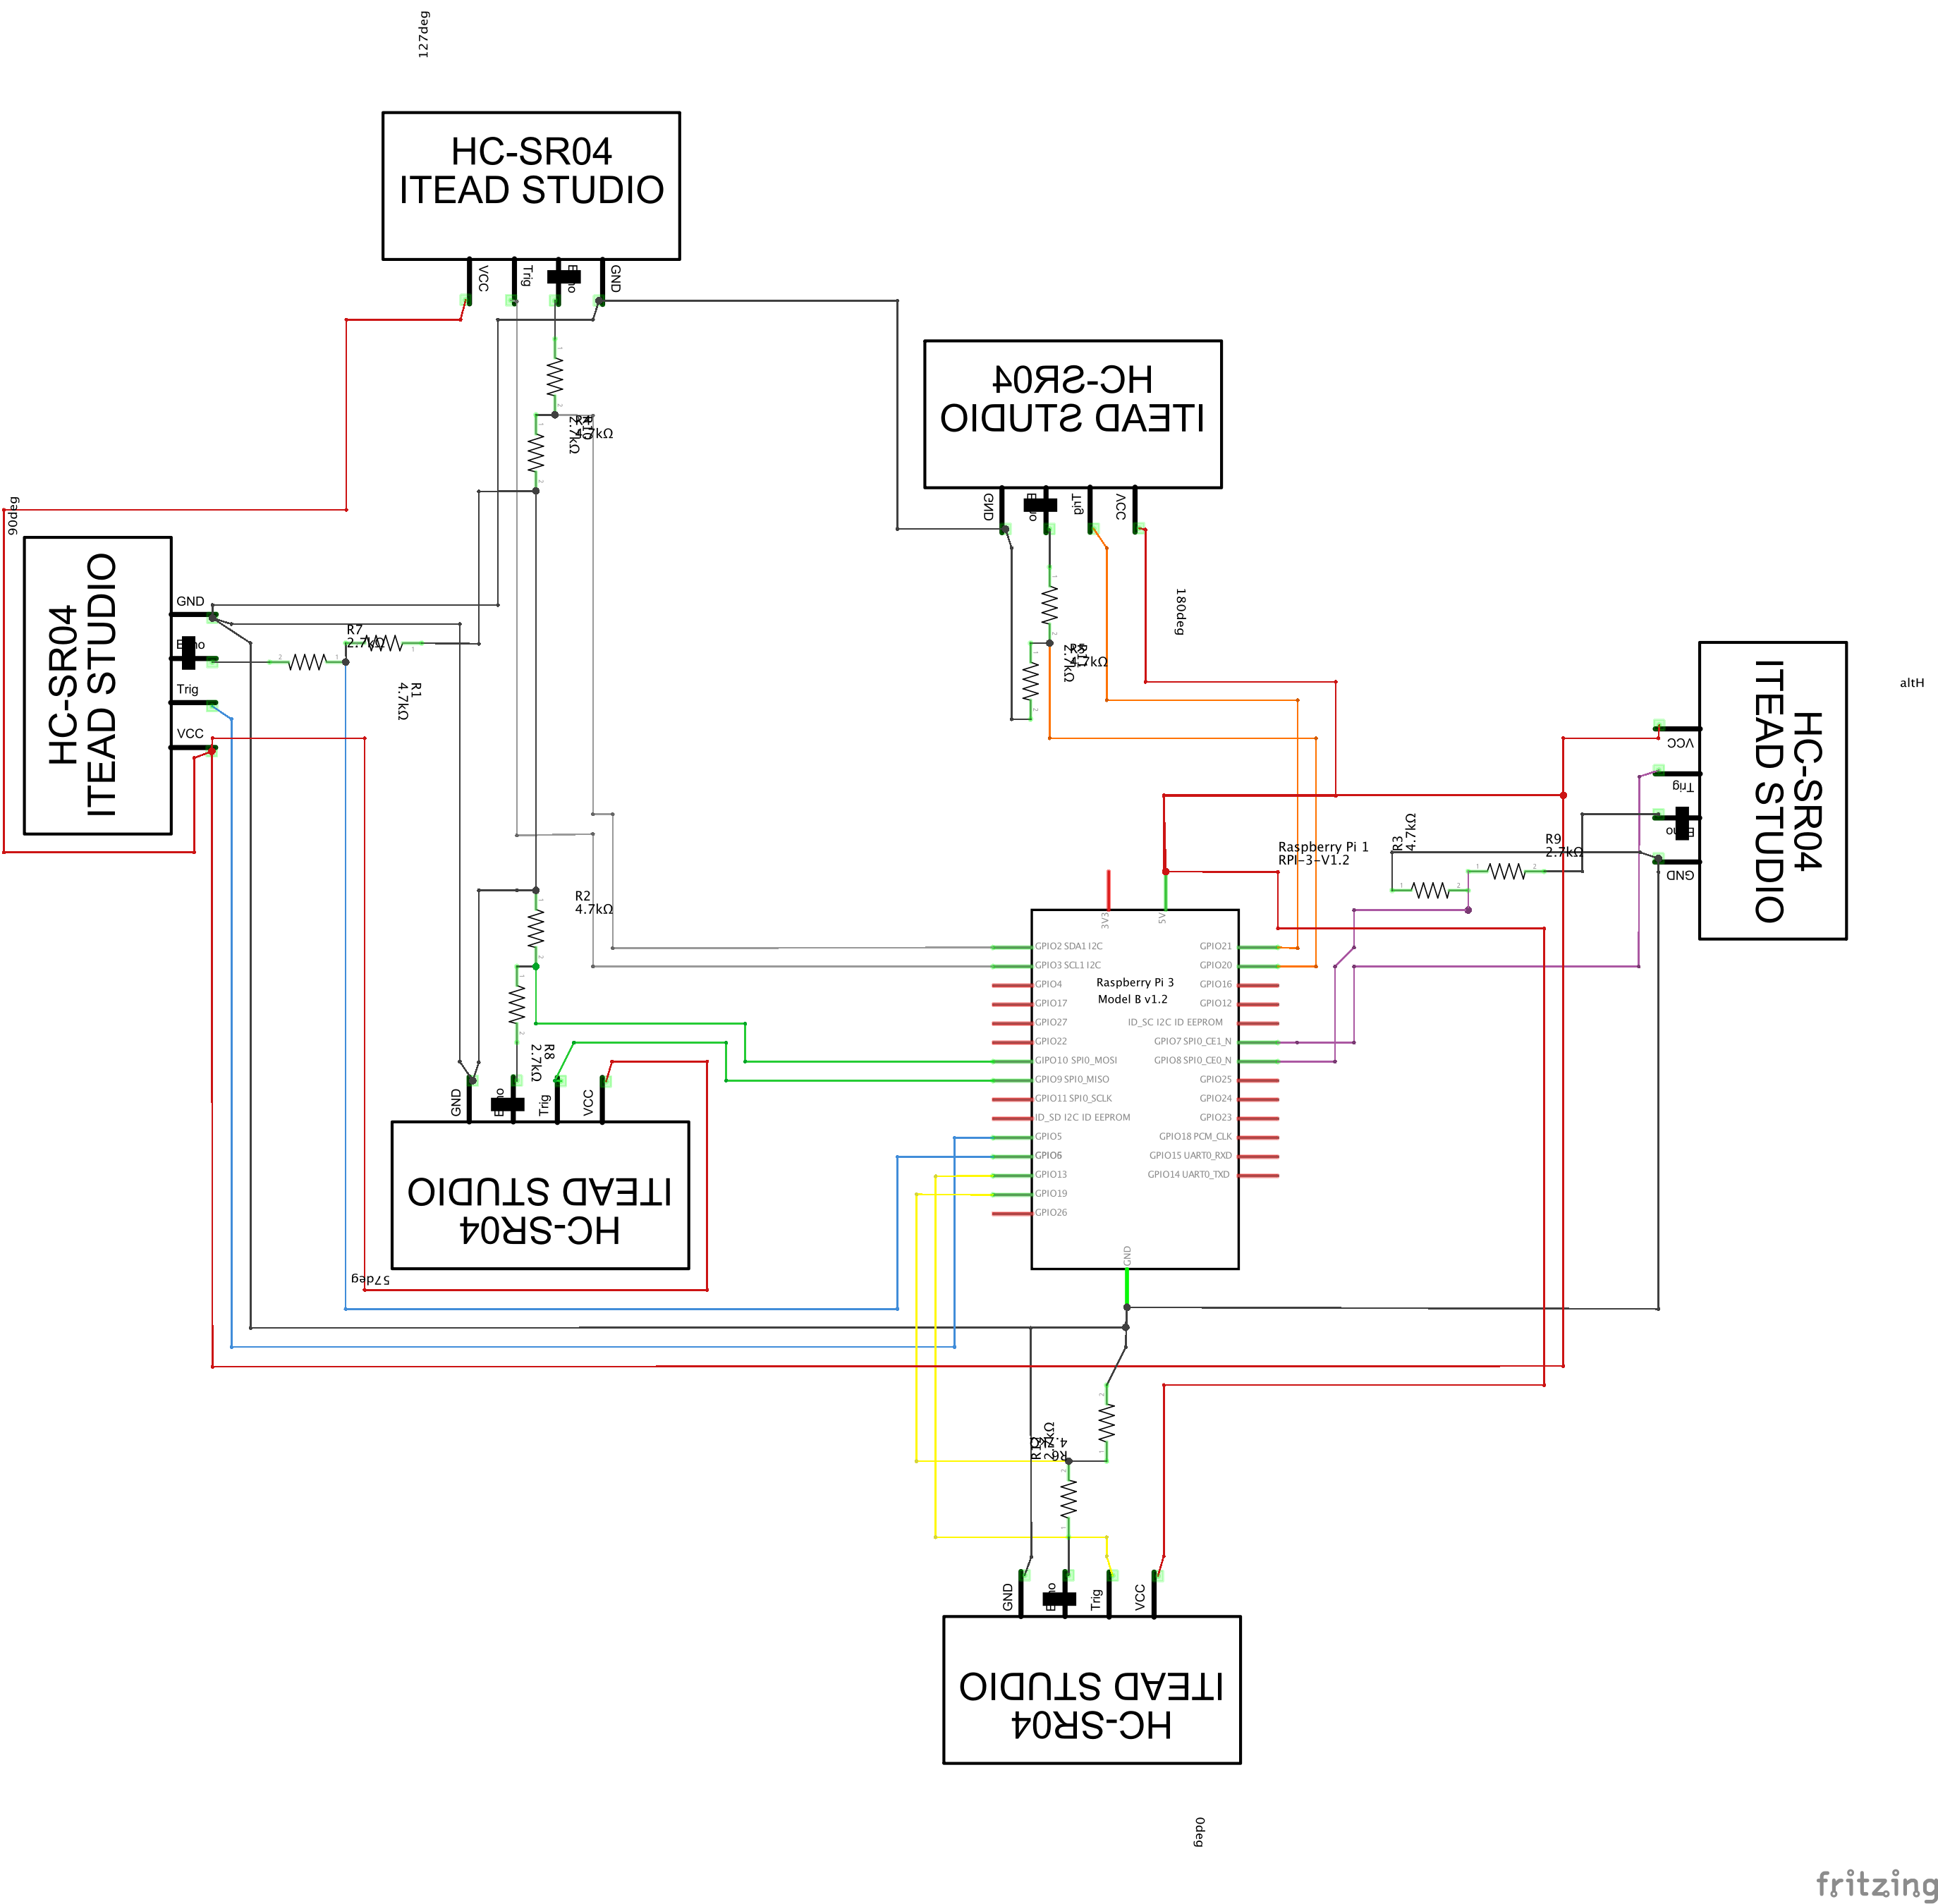
\includegraphics[width=0.9\textwidth]{SR04layout_schem}
	\caption[Diagrama de conexión de sensores a RaspberryPi]{Vista esquemática del conexionado de los sensores a la RaspberryPi.}\label{fig:concepHCPi}
\end{figure}

\begin{figure}
	\centering
	\includegraphics[width=0.75\textwidth]{voltDivider}
	\caption[Divisor de voltaje]{Vista imagen de los divisores de voltaje creados.}\label{fig:imgVoltDiv}
\end{figure}

\begin{figure}
	\centering
	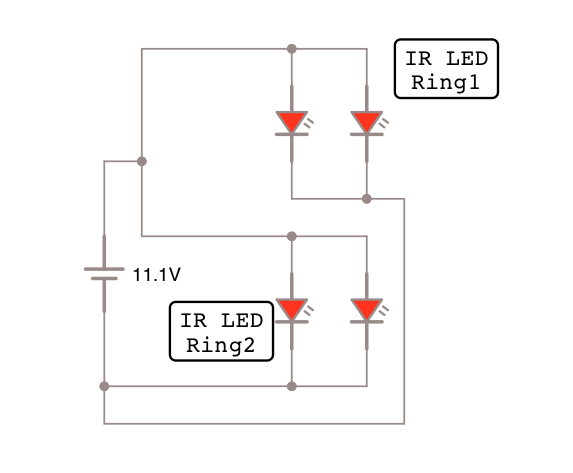
\includegraphics[width=0.6\textwidth]{IRLED}
	\caption[LED IR]{Vista esquemática del conexionado de los LED Infrarrojos.}\label{fig:schIRLED}
\end{figure}

\begin{figure}
	\centering
	\includegraphics[width=0.9\textwidth]{droneSide}
	\caption[Lateral del \emph{drone}]{Detalle del \emph{drone} completo. Lateral.}\label{fig:droneSideView}
\end{figure}

\begin{figure}
	\centering
	\includegraphics[width=0.9\textwidth]{droneFront}
	\caption[Frontal del \emph{drone}]{Detalle del \emph{drone} completo. Frontal.}\label{fig:droneFrontView}
\end{figure}


\section{Pruebas}
\label{sec:testing}
Sin duda la parte más relevante del proyecto es la implementación física del mismo. Las pruebas llevadas a cabo se han centrado en la componente práctica, y en pruebas de campo. 

Las diferentes clases desarrolladas han sido testadas de forma interna, y no se dispone de pruebas como tal, que puedan ser desplegadas en un sistema de integración continua. 
La motivación de no realizar este tipo de pruebas es la siguiente: 
\begin{itemize}
\item Las pruebas relacionadas con la comunicación entre el \emph{drone} y la RaspberryPi requieren de una controladora de vuelo, y hacer un \emph{mock} de este componente, supondría tener que estudiar la implementación completa que ofrece una controladora de vuelo al protocolo MultiWiiSerialProtocol, así como de todos los sensores. De no hacerlo, no existen sistemas de integración que pongan a nuestra disposición una controladora, un equipo que abra un puerto serie y que ejecute una serie de comandos/solicitudes interpretables por dicha controladora. Se incluye una pequeña clase de prueba que permite comprobar si se adquieren correctamente los datos de la controladora de vuelo, dibujando un plot de los ejes de inclinación y orientación, tal y como puede verse en la Figura \ref{fig:mspIMU}, y en el vídeo \href{https://universidaddeburgos-my.sharepoint.com/:v:/g/personal/mbm0089_alu_ubu_es/EezmUjB1BSdKp-_VQrUkIXwBPSrvQdSnmhSTd-QA3jJaIQ?e=RYEaIl}{V\#1}.
\begin{figure}
	\centering
	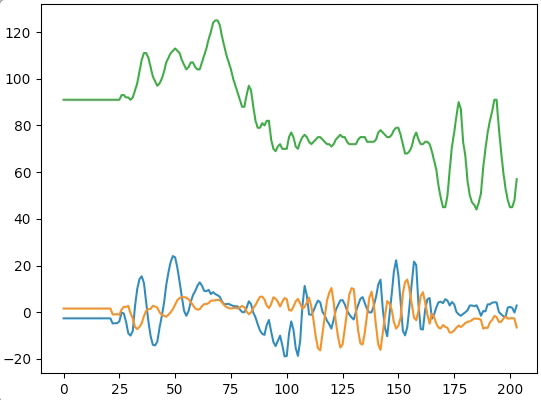
\includegraphics[width=0.9\textwidth]{mspIMU}
	\caption[Recepción de la IMU mediante MSPio]{Salida de los sensores de la controladora de vuelo. En azul la elevación, en naranja el balanceo y en verde la orientación.}\label{fig:mspIMU}
\end{figure}


\item De igual manera sucede con el sistema de control Remoto, que depende de la controladora de vuelo para comprobar su completo funcionamiento. De testearlo de forma parcial, solo se conseguiría comprobar que los paquetes llegan de forma correcta hasta el destino, y esta prueba se ha realizado como parte de las pruebas de campo, ver subsección \ref{subsec:fieldTestingv1}, de forma satisfactoria, ya que ayudó a corregir un \emph{bug} de difícil detección.
\item Las pruebas relacionadas con el sistema de evasión de obstáculos, requieren de los diferentes sensores de distancia, de nuevo no existe ningún sistema de integración que proporcione dicho hardware. Realizar un mock de dichos sensores supone perder por completo la dinámica del sistema, i.e, los sensores no son perfectos, dan medidas con ruido, el \emph{drone} no siempre se moverá con perfección milimétrica, los sensores no están perfectamente alineados, etc. Se realizaron pruebas durante su desarrollo mediante mock de los sensores, la cual puede ejecutarse si se utiliza la clase del VFH como \code{\_\_main\_\_}.
\item Las pruebas relacionadas con el sistema de localización están basadas en los mismos sensores anteriores. El mock de dichos sensores para esta clase caería en una sobresimplificación del sistema, tal y como ocurre en el curso de UdaCity, ver \citep{wiki:UdCityPF}, que solo daría una sensación de falsa funcionalidad del sistema. Realizar pruebas sobre el funcionamiento base del Filtro de Partículas no es relevante, ya que no existe la dinámica encontrada en un entorno real. Pese a ello, en la clase que representa el Filtro de Partículas, se encuentra una pequeña prueba de su funcionamiento para un pequeño mapa en el que existen tres obstáculos. La dimensionalidad que alcanza el filtro es tal, que durante las pruebas no es nada sencillo apreciar el recorrido del algoritmo. De igual manera existe una pequeña prueba en la clase que representa los cálculos geométricos requeridos para el Filtro de Partículas.
\end{itemize}


\subsection{Pruebas de Campo}

Las pruebas de campo han permitido demostrar el funcionamiento del \emph{drone}, así como encontrar errores en la programación. Se han mostrado de gran utilidad, no solo en la búsqueda de errores, sino como fuente de información para futuras mejoras, así como para proyectos derivados o complementarios a este.

Esta sección se ha dividido en dos subsecciones, cada una establecida en base a la \emph{release} a la que hacen referencia las pruebas. 


\subsubsection{Primera Release: v0.1.0-alpha}
\label{subsec:fieldTestingv1}

Las primeras pruebas de campo llevadas a cabo, se realizaron en el polígono industrial de Villalonquejar, en Burgos. 
Dado que la primera \emph{release} no incluye ningún elemento de automatización, sino que comprende el apartado relacionado con el control remoto del \emph{drone}, pudieron ser llevadas a cabo sin demasiados inconvenientes en una zona apartada, pero no cerrada. 

\begin{figure}
	\centering
	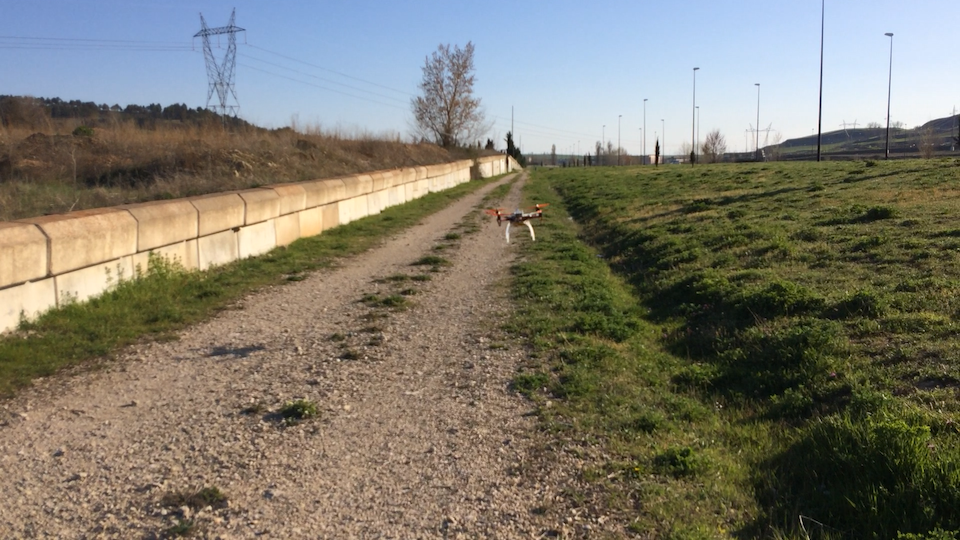
\includegraphics[width=0.9\textwidth]{ftest1}
	\caption[Field Test 1. Villalonquejar]{Drone despegando durante la primera prueba de campo.}\label{fig:ftest1Drone}
\end{figure}

La comunicación con el \emph{drone} se estableció creando un punto de acceso desde un ordenador portátil. Seguidamente, se inició el servidor web en el portátil, el sistema de control del \emph{drone}, y servidor WebRTC ambos en la RaspberryPi. El resultado de las pruebas puede verse en el vídeo \href{https://universidaddeburgos-my.sharepoint.com/:v:/g/personal/mbm0089_alu_ubu_es/ERit03PQ4GVJvVXNLCxQQwUBUjZt6VjCwl5GcLUYwFQGPQ?e=dD258g}{V\#3}.

Las pruebas comprenden los siguientes apartados, puntuados según la calidad del resultado en una escala de $(0, 10]$: 
\begin{itemize}
\item Comprobación del correcto despliegue del sistema en una situación real: El despliegue se efectúa sin problema, la RaspberryPi responde correctamente a la comunicación vía SSH. Se realiza el despliegue perfectamente haciendo uso de la herramienta de \emph{deployment} de que provee el IDE PyCharm. 10/10.
\item Comprobación del sistema de vídeo en tiempo real: La comunicación con el servidor WebRTC es perfecta en este sentido. No existen retardos alarmantes en el feed de vídeo con una resolución de $1280 \times 720$ a $15f/s$. Reducir la resolución y aumentar los fps podría ser una solución mejor, aunque el sistema no se moverá a una velocidad alta. La calidad del vídeo, sin embargo, es cuestionable. Al tratarse de una cámara sin filtro de luz infrarroja, los colores parecen algo saturados en ocasiones.  9/10.
\item Comprobación del sistema de login, web y comunicación con el \emph{drone}: El login se realiza de forma correcta, se reconoce el \emph{drone} asignado al usuario y se activa la comunicación con este sin problema. 10/10.
\item Comprobación del sistema de control remoto en tiempo real: El sistema de control remoto se activa sin problema, la comunicación es relativamente fluida, el \emph{drone} responde correctamente a los comandos enviados, aunque con cierta latencia. Cabe destacar que los mensajes viajan hasta el servidor web que posteriormente se encarga de enviarlos al \emph{drone}. 
Se encuentra un \emph{bug}, referenciado en la \emph{issue} \href{https://github.com/mbm0089/GII_0_17.02_SNSI/issues/53}{\#53}, existente a la hora de \emph{parsear} el paquete JSON recibido por el servidor de control remoto existente en el \emph{drone}. La recreación del \emph{bug}, puede verse en el vídeo \href{https://universidaddeburgos-my.sharepoint.com/:v:/g/personal/mbm0089_alu_ubu_es/ERit03PQ4GVJvVXNLCxQQwUBUjZt6VjCwl5GcLUYwFQGPQ?e=dD258g}{V\#3} a partir del minuto 3:32. 
El \emph{bug} detectado se debía a la debilidad de la señal al alejarse el \emph{drone} del punto de acceso, ocasionando la pérdida de paquetes.
\end{itemize}

La realización de las pruebas ha dado como resultado la valoración de la release \emph{v0.1.0-alpha} como lista para ser publicada. Sin embargo se mantiene como versión \emph{alpha} dada la necesidad de realizar todavía más pruebas. 
Gracias al \emph{bug} detectado, y solucionado, se valora incluir en la RaspberryPi una antena wifi mejor que la existente, o proporcionar a la RaspberryPi un modem 4G conectado vía USB para mantener siempre comunicación con el servidor. De esta forma se reducen las probabilidades de perder paquetes. 


\subsubsection{Segunda Release: v0.2.0-alpha}
\label{subsec:fieldTestingv2}

La segunda release del proyecto, traerá las siguientes mejoras y características sobre la anterior versión:
\begin{itemize}
\item Grabación del feed de vídeo en el ordenador cliente, haciendo uso de WebRTC.
\item Inclusión de diferentes sistemas de control automatizado, establecidos mediante un sistema de prioridades.
\item Automatización del control de altitud.
\item Automatización del control de velocidad.
\item Automatización del control de dirección.
\item Localización sin GPS.
\item Evasión de obstáculos.
\item Seguimiento de rutas.
\end{itemize}

Las pruebas realizadas comprenden los siguientes apartados, puntuados según la calidad del resultado en una escala de $(0, 10]$. Dada la peligrosidad de algunas de las pruebas, se ha llevado el \emph{drone} a una nave industrial, ver agradecimientos en \ref{sec:agradecimientos}, dado que provee de un entorno seguro y cerrado en el que probar mecanismos automatizados:
\begin{figure}
	\centering
	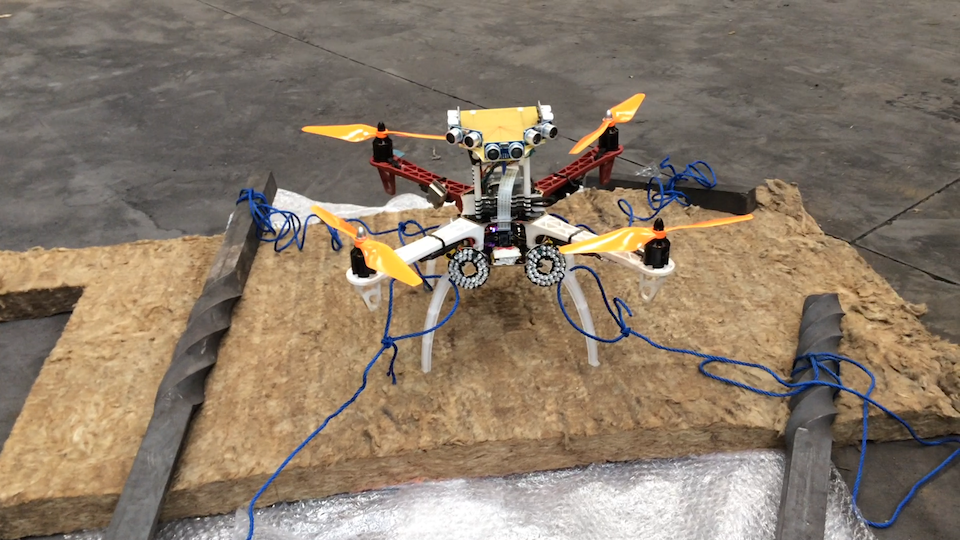
\includegraphics[width=0.7\textwidth]{ftest2init}
	\caption[Field Test 2. Nave industrial]{Drone sobre superficie blanda durante el segundo field test}\label{fig:ftest2init}
\end{figure}

\begin{itemize}
\item Calibrado del sistema de control de altitud: Se trata de un controlador PID que debe ser parametrizado. Dada la dinámica del sistema, tan dependiente del estado de la batería, de los cambios de contexto realizados por el sistema (recordemos que no es un RTOS\footnote{Real Time Operative System}), de los errores de medida proporcionados por el sensor, etc. La parametrización del PID ha sido bastante compleja. De hecho durante el transcurso de las pruebas, se rompió una hélice y una de las patas que hacían de apoyo para el \emph{drone}, dificultando esto último, todavía más, el proceso de estabilización durante el despegue. 
\begin{figure}
	\centering
	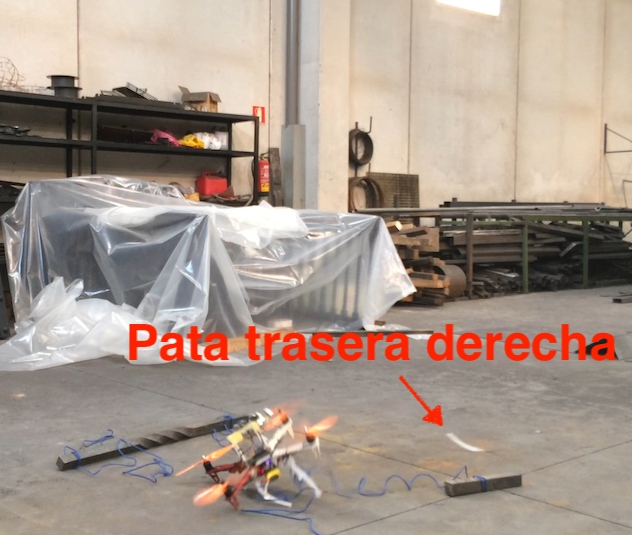
\includegraphics[width=0.7\textwidth]{ftest2cripple}
	\caption[Field Test 2. Demasiada kP]{Drone perdiendo una pata.}\label{fig:ftest2cripple}
\end{figure}
\begin{figure}
	\centering
	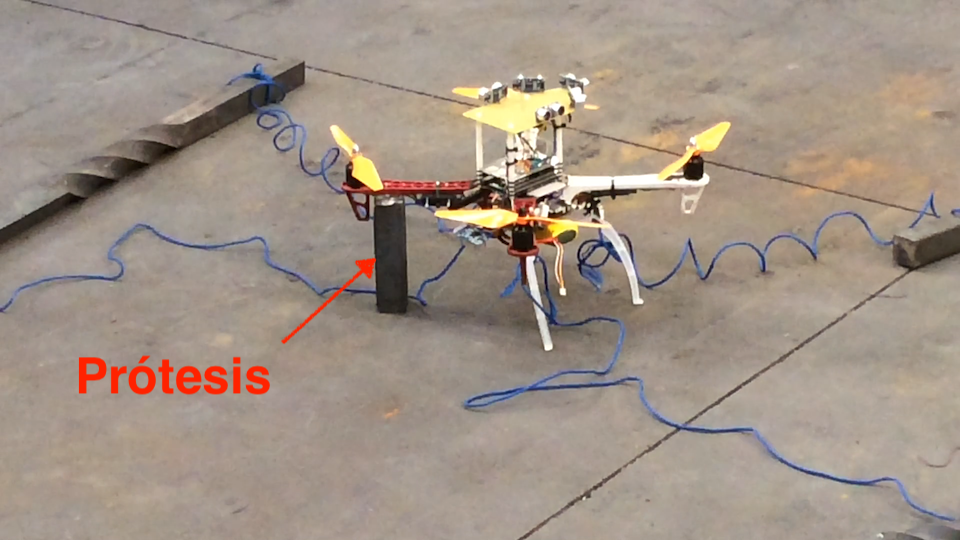
\includegraphics[width=0.7\textwidth]{ftest2newleg}
	\caption[Field Test 2. Prótesis]{Drone con prótesis.}\label{fig:ftest2newleg}
\end{figure}

La motivación para retirar el material blando que puede verse en la Figura \ref{fig:ftest2init}, es que es tan absorbente que falseaba las medidas tomadas por el sensor de ultrasonidos.

En el vídeo \href{FALTA REF!!!}{V\#4} puede verse el proceso llevado a cabo. 

Se detectó un \emph{bug} existente en el cálculo del PID que llevaba a la pérdida de precisión al realizar una conversión a entero, antes de realizar redondeo. Esto podía causar que el error acumulado se disparase, y por lo tanto dar a la componente Integral del sistema una importancia no deseada. Dado que se trata de un \emph{bug} menor, se solucionó \textit{in situ} por lo que no se generó una issue para ello.

Se detectó un \emph{bug} existente en el sistema de control que no permitía que un controlador automatizado controlase cuándo armar el \emph{drone}. Esto produciría que el sistema de control de altitud, no pudiese actuar. Se trata de un \emph{bug} menor, basado en añadir una pequeña espera en la que se mantiene la entrada del canal 5 (armar/desarmar) a un valor mínimo durante unos segundos, a la espera de que el sistema calibre el acelerómetro y el giróscopo. Solucionado \textit{in situ}, no se ha generado una issue para ello.
 El resultado de las pruebas de altitud no ha sido el deseado. No se ha conseguido que el \emph{drone} mantenga la altitud de forma correcta. Si que la alcanza sin problema, pero requiere de ajustar más los parámetros del controlador PID.
 \begin{figure}
	\centering
	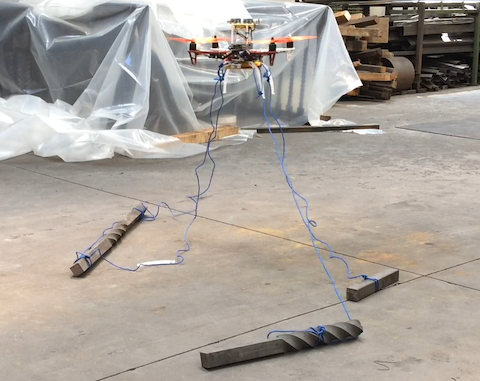
\includegraphics[width=0.7\textwidth]{ftest2altH}
	\caption[Field Test 2. Altura alcanzada con suavidad]{El \emph{drone} alcanza con relativa suavidad la altura, pero no la mantiene correctamente.}\label{fig:ftest2heightreached}
\end{figure}
 
Sin embargo ha arrojado claridad sobre ciertos problemas, y mejoras que se deberían probar. 5/10.
 
 \item Calibrado del sistema de control de velocidad: La velocidad a adquirir por el \emph{drone} se basa en la inclinación del mismo. Se trata, de nuevo, de un controlador PID que debe ser parametrizado. Dada la imposibilidad de mantener la altura de forma correcta, y la indudable peligrosidad de este test, se ha preferido postergar la realización de estas pruebas hasta que se haya dado con una parametrización correcta del control de altitud. 0/10.
 
 \item Calibrado del sistema de control de dirección: La dirección a seguir se basa en la orientación del \emph{drone}. Se trata, de nuevo, de un controlador PID que debe ser parametrizado. Dada la imposibilidad de mantener la altura de forma correcta, y la indudable peligrosidad de este test, se ha preferido postergar la realización de estas pruebas hasta que se haya dado con una parametrización correcta del control de altitud. 0/10.
\end{itemize}


La realización de las pruebas ha dado como resultado la valoración de la release \emph{v0.2.0-alpha} como \textbf{no} lista para ser publicada. Sin lugar a dudas, requiere de muchas más pruebas en un entorno controlado antes de poder plantear la posibilidad de liberar esta versión. 

Dados los resultados de las pruebas, convendría valorar los siguientes cambios en la estructura del \emph{drone}: 
\begin{itemize}
\item Reducir el peso total del dispositivo. Puede utilizarse una estructura de carbono, o similar.
\item Mejorar el control de estabilidad del \emph{drone}. Parece que la controladora de vuelo Flip32 no es lo ideal para este tipo de \emph{drone} tan pesado y grande. Podría valorarse la posibilidad de cambiar a una controladora más moderna, y realizar una calibración de los PID mucho más acertada. De hecho la controladora de vuelo es, en términos tecnológicos, antigua.
\item Cambiar los sensores de altitud, por uno con una tasa de adquisición mucho mayor. Este es uno de los principales problemas del cálculo del PID. El cuello de botella del sistema no está en el hecho de usar Python o de que no se trate de un sistema operativo de tiempo real, sino en la lentitud de los sensores. Los HC-SR04 requieren de un tiempo para tomar sus medidas demasiado elevado, unos $0.06s$, lo cual quiere decir que el número de veces por segundo que se calcula el PID no es elevado. Por ello, la salida proveniente del cálculo del PID es difícil de ajustar, ya que pueden darse variaciones relativamente grandes entre las medidas tomadas por los sensores. Se tiene que limitar la frecuencia del cálculo de PID a la tasa de adquisición de medidas del sensor, dejando una frecuencia de muestreo de, como máximo, 16Hz en el caso del sensor de altitud. 
\item Para evitar ecos, el `disparo' de ultrasonidos se realiza de forma secuencial, no enviando el siguiente disparo hasta que el anterior sensor haya recibido su medida. Dada la lentitud de estos sensores y que existen 5 de ellos en el cálculo de distancia a obstáculos, tomar una sola medida llevaría $0.06s \times 5 = 0.3s$. De esta forma, la frecuencia de muestreo, y por tanto del cálculo del PID, cae a tan solo 3Hz. Esta cantidad de tiempo, puede tornarse inaceptable en el momento en el que el sistema se desplace a una velocidad mayor, o requiera de mayor precisión. Por tanto se sugiere cambiar estos sensores por un sensor de distancia mucho más preciso y rápido, una solución basada en LIDAR debería ser valorada, o incluso en cámaras, dado el aumento de la capacidad de cómputo de las RaspberryPi.
\end{itemize}




\section{Agradecimientos}
\label{sec:agradecimientos}

Casi 90 páginas de memoria, sin contar anexos, y un montón de horas de lectura y búsqueda de información no podían pasar sin una, breve, sección de agradecimientos: 

\begin{itemize}
\item En primer lugar a Laura, que me animó a comenzar esta carrera hace cuatro años, y que nunca ha dejado de animarme.
\item A mi padre, que también es uno de mis mejores amigos, y ha sabido animarme (y aguantarme) en cualquier momento de frustración. 
\item A mis tres tutores Alejandro, Jose y César, que han gestionado este proyecto de forma impecable, y me han asesorado ante cualquier eventualidad. Me gustaría haber podido hacer más y dejarlo completado.
\item A David, mi mejor amigo, que siempre me anima a inventarme cosas nuevas, y que siempre tiene unas palabras de ánimo para mí. 
\item A Isaac, otro gran amigo, y mi cámara durante la primera sesión de pruebas, ver subsección \ref{subsec:fieldTestingv1}.
\item A Cerrajería Artística Gutiérrez, por dejarme usar un espacio en su nave en Aranda de Duero para la segunda sesión de pruebas, ver subsección \ref{subsec:fieldTestingv2}. De no ser por ellos, hoy seguiría tratando de bajar el \emph{drone} de algún árbol.
\end{itemize}

















